\documentclass[11pt]{article}
\usepackage[a4paper,landscape,margin=12mm]{geometry}
\usepackage{graphicx}
\usepackage{lmodern}
\pagestyle{empty}
\begin{document}
\noindent\centering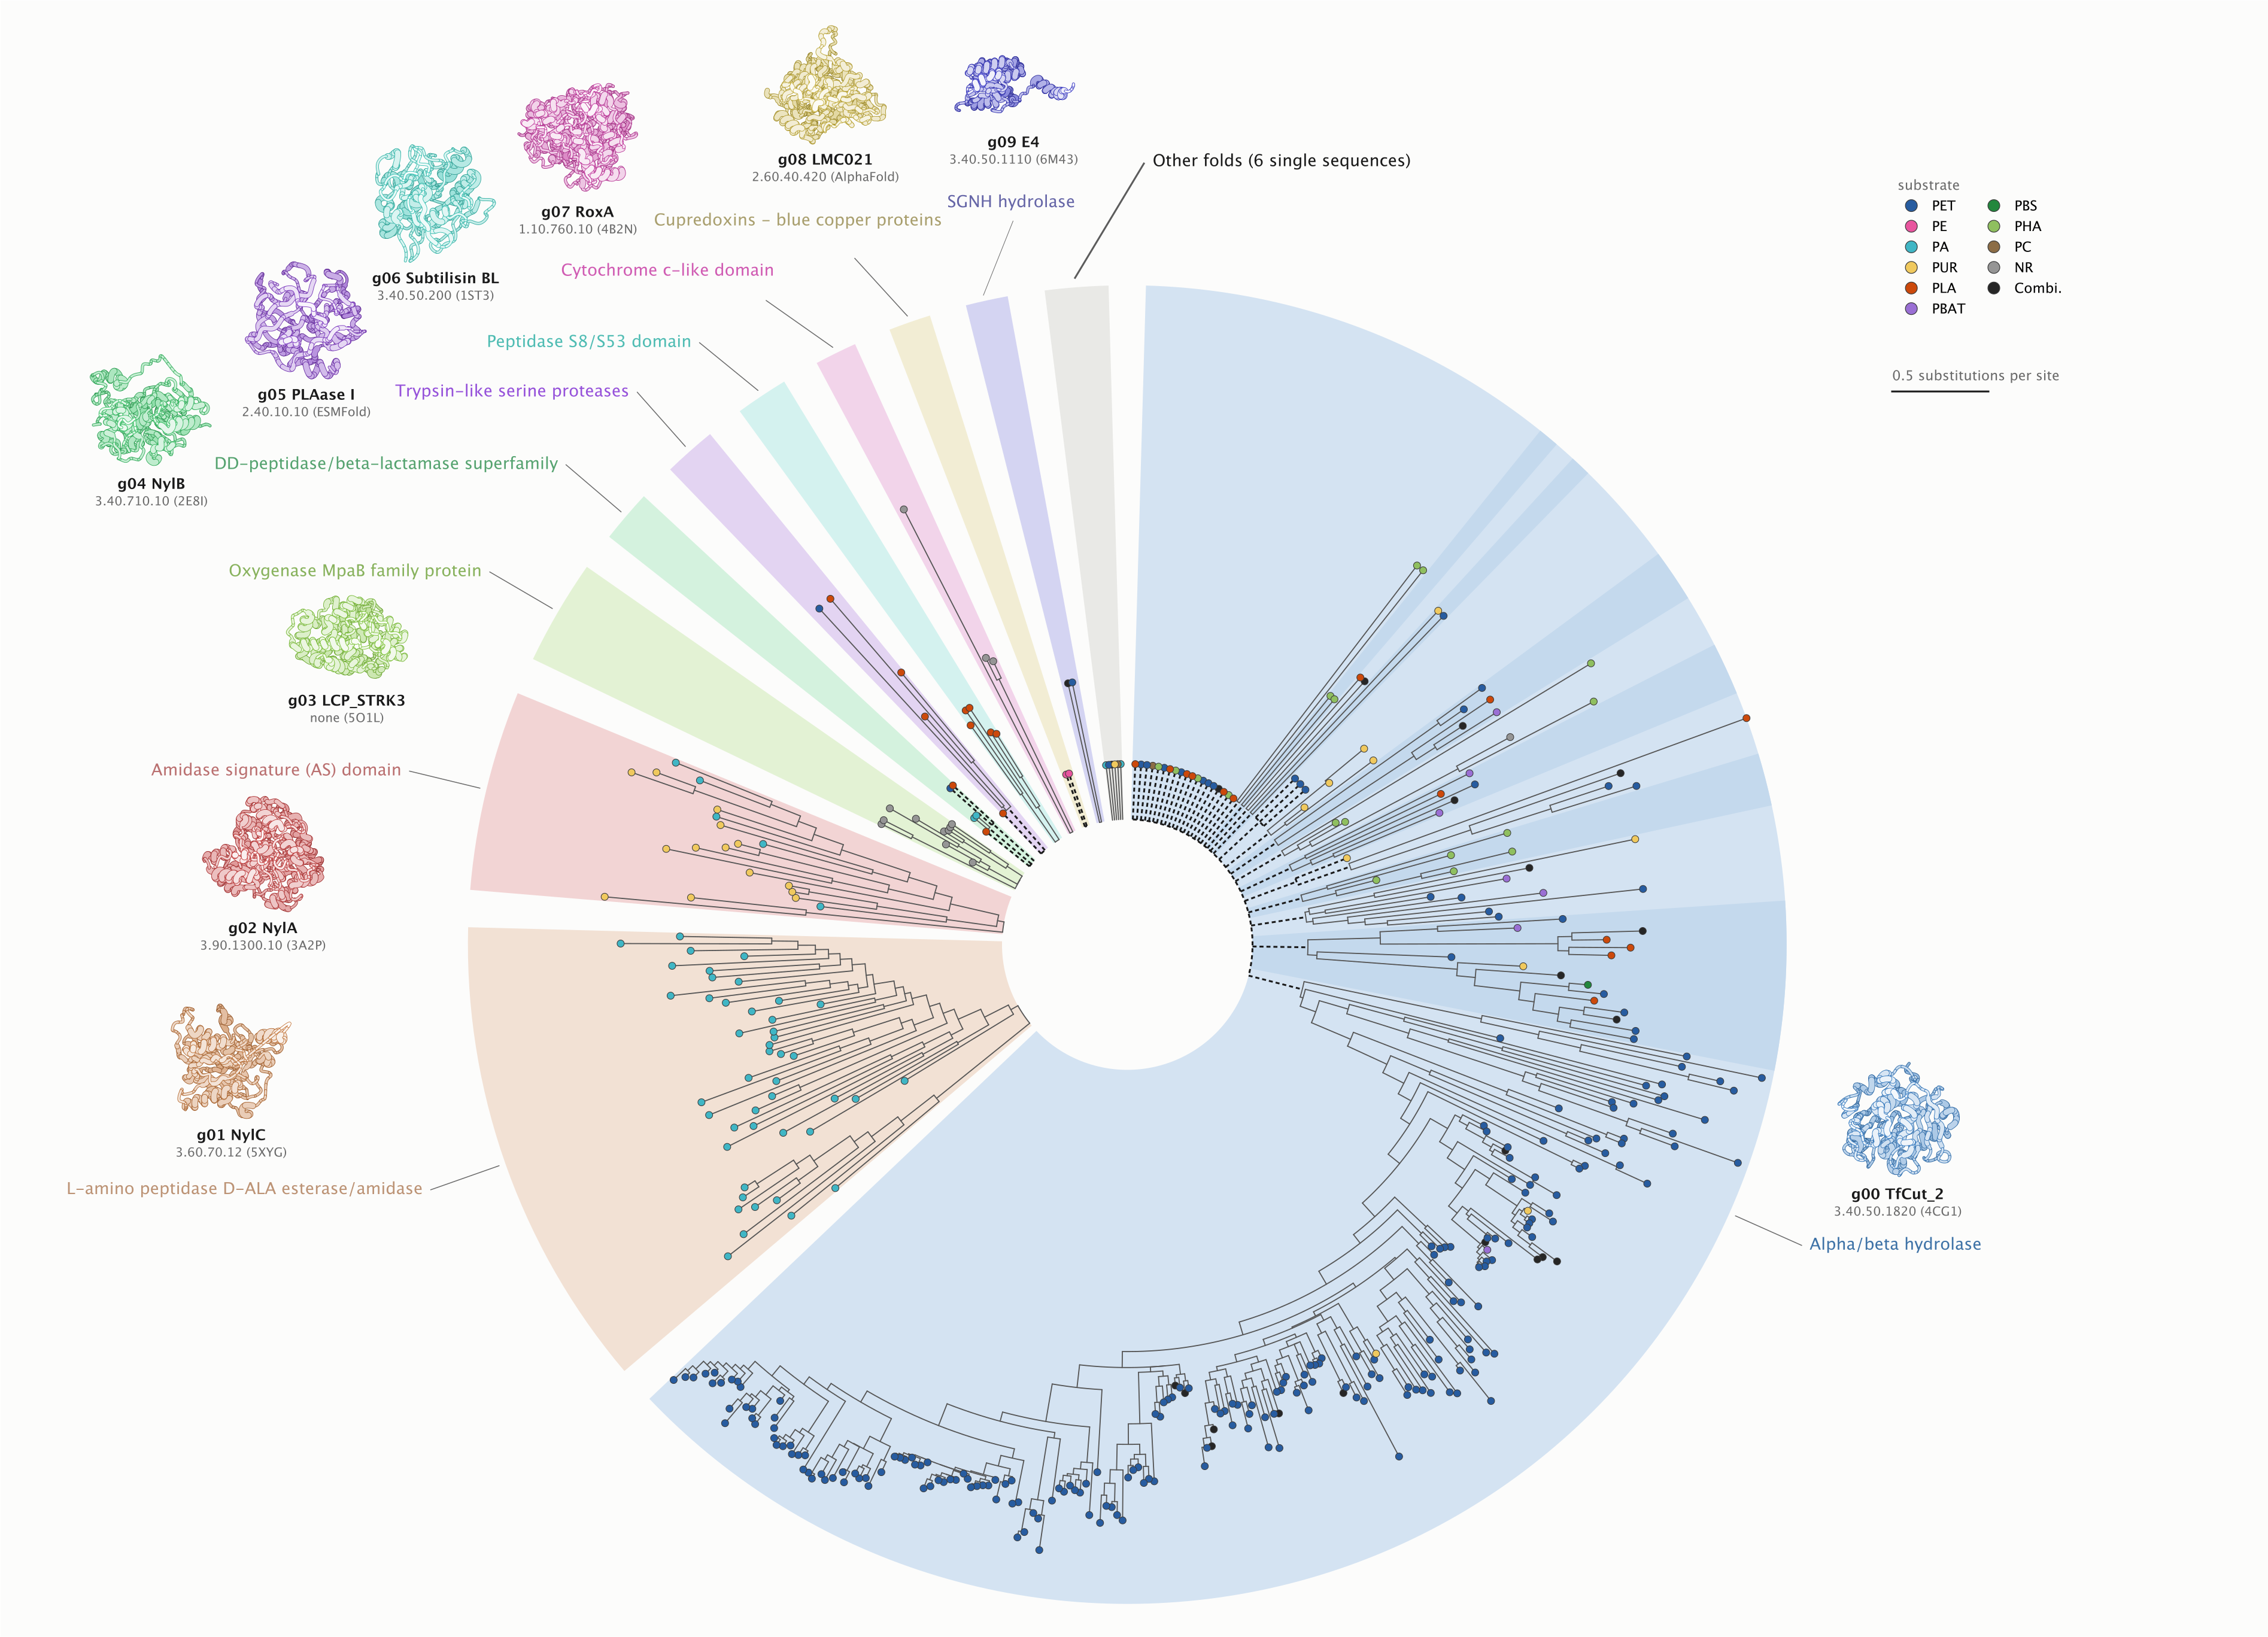
\includegraphics[height=135mm]{../figures/figure2c_plasticome-forest.png}\par\raggedright

\vspace{4mm}
\noindent\textbf{Supplementary Fig.~1. The plasticome as a forest of fold groups.} The 411 plasticome centroids in 56 sequence-similarity families (connected components at 30\% identity over 50\% coverage), grouped into 16 fold groups by the CATH superfamily of their catalytic domain. Each slice is one fold group with its own tree; slices are not related to each other. Tips are coloured by substrate; dashed lines are supported links between families of the same fold (not to scale). Structures show one representative enzyme per fold, with its CATH superfamily and PDB entry; LMC021 (AlphaFold DB) and PLAase I (ESMFold) are predicted models.
\end{document}
